\chapter{Evaluation}
\label{chapter:evaluation}
\thispagestyle{myheadings}

% set this to the location of the figures for this chapter. it may
% also want to be ../Figures/2_Body/ or something. make sure that
% it has a trailing directory separator (i.e., '/')!
\graphicspath{{./5_Evaluation/}}

\section{Optimality checking}
Now we have learnt a model $Q_{\theta}$, we also have our test cases $\{(x_{i},y_{i})\}_{i\in[n]}$.\\
Each data window corresponds to $24$ data entries. The $t^{th}$ window corresponds to 
$$\{x_{24t}, x_{24t+1}, ..., x_{24t+23}|t\in\mathbb{I}\}$$
Each data window has $24$ data points as we have tried all possible($24$ of them) combinations of ordering of operations. For each data window we need to find the ordering of operations which requires the minimum moves according to our predictions.\\
To do this for the $t^{th}$ window of data, find the index of the minimum of $$Q_{\theta}(x_{24t}),Q_{\theta}(x_{24t+1}),...,Q_{\theta}(x_{24t+23})$$, say $k$.\\
To check if the move this corresponds to is the actual optimal move, find the index of the minimum of $y_{24t}, y_{24t+1}, ..., y_{24t+23}$, say $l$. If $k=l$ then the move we predicted as optimal is indeed optimal.\\ 
\par We train the model multiple times on the training data and measure its performance on the test data each time.\\
To measure the performance we use the predicted optimal move vs the actual optimal move.\\

\section{Justification}
The things considered while determining the neural network to use for training the DQN are :-
\begin{itemize}
    \item To achieve a value as close as possible to the global minima for the optimization function (Adam optimzer)
    \item The time required to predict the optimal move should not exceed the time saved by using it.
    \item The time and resources required for training should not exceed the capacity of the system while it is running the query processing in the background. 
\end{itemize}
What we found was:-
\begin{itemize}
    \item Adding additional layers improve the prediction of the optimal moves but not by significant margin.
    \item Adding additional layers resulted in the time spent predicting the answer overshadowing the time saved by executing the optimal move.
\end{itemize}
\par But note, these $2$ are only query and data specific findings.

\section{Results}
In this section, we present:-
\begin{itemize}
    \item The frequency distribution of the entire dataset.
    \item Present our confusion matrix, heat map and the values extracte from it.
    \item Analyse various predictions for various classes.
    \item Present how our model performed compared.
\end{itemize}


\subsection{Data Distrbution}
As visible from the below diagram \ref{fig:totalb1} the disparity in the frequency distribution is massive. Learning a model based on biased data is often difficult as the smaller classes tend to be ignored. As visible the data is higly biased towards the last $2$ orderings.\\

\begin{figure}
\centering
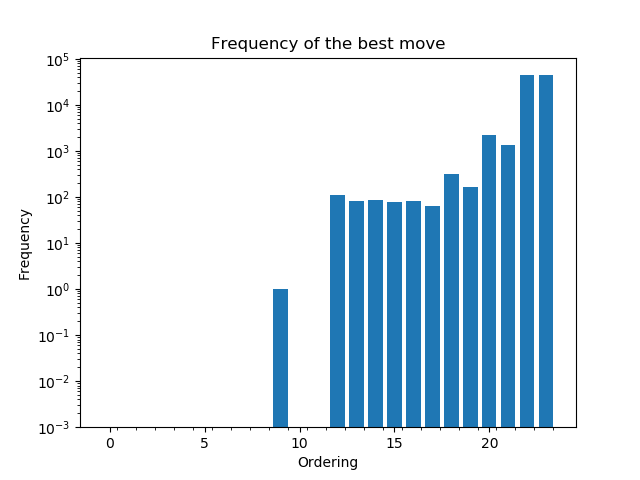
\includegraphics[scale=0.75]{totalb1.png}\\
\caption{This figure shows the frequency distribution of the number of cases where each move is optimal}
\label{fig:totalb1}
\end{figure}

The actual values of the above distribution are presented here\ref{lst:total_data}.

\begin{lstlisting}[caption=Frequencies of optimal moves in total data, label={lst:total_data}]
[0, 0, 0, 0, 0, 0, 0, 0, 0, 1, 0, 0, 110, 83, 84, 79, 80, 63, 307, 165, 2209, 1367, 43849, 43872]
\end{lstlisting}

\par For training purposes, we divided the data in $70\%$ for training and $30\%$ for testing. Cross validation did not have a significant impact on training parameters nor on the results for prediction of test data. We visualized the training and testing data below \ref{fig:trainingb1} and \ref{fig:testingb1}

\begin{figure}
\centering
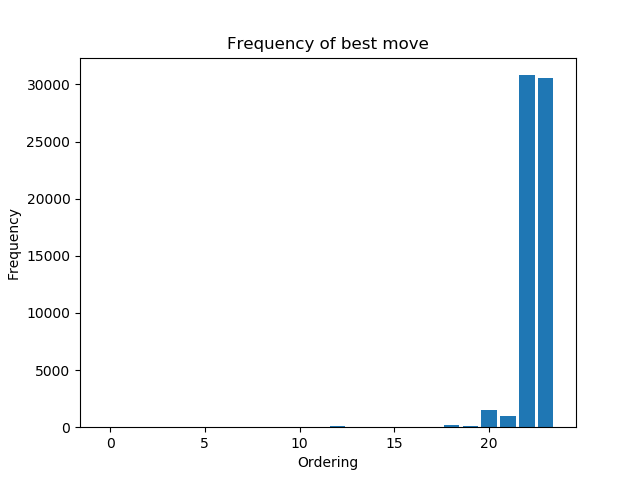
\includegraphics[scale=0.75]{trainingb1.png}\\
\caption{This figure shows the frequency distribution of cases where each move is optimal in the training dataset}
\label{fig:trainingb1}
\end{figure}

\begin{figure}
\centering
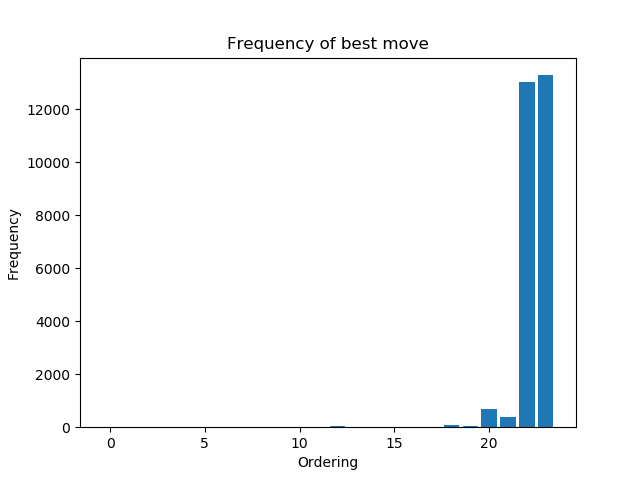
\includegraphics[scale=0.75]{testingb1.png}\\
\caption{This figure shows the frequency distribution of cases where each move is optimal in the testing dataset}
\label{fig:testingb1}
\end{figure}

The actual values for the frequency distribution are given in \ref{lst:training_data} and \ref{lst:testing_data}

\begin{lstlisting}[caption= Frequencies of optimal move in training data, label={lst:training_data}]
[0, 0, 0, 0, 0, 0, 0, 0, 0, 0, 0, 0, 81, 60, 59, 54, 57, 45, 227, 119, 1526, 966, 30811, 30583]
\end{lstlisting}
\begin{lstlisting}[caption= Frequencies of optimal move in testing data, label={lst:testing_data}]
[0, 0, 0, 0, 0, 0, 0, 0, 0, 1, 0, 0, 29, 23, 25, 25, 23, 18, 80, 46, 683, 401, 13038, 13289]
\end{lstlisting}


\subsection{Confusion matrix}
\textbf{Confusion matrix} or error matrix is a table that aids with visualizing the performance of an algorithm, usually a supervised algorithm, in this case for classificaiton purpose. Each row of the matrix represented a class, specifically meant to represent the predicted class by the classification algorithm, while the column is meant to represent the actual class. \\
In the confusion matrix $\mathbb{A}$, the entry $\mathbb{A}[i,j]$ is interpretted as, the number of data points of class $j$ predicted to be $i$.
\par As we trained the DQN over multiple iterations, we present two of it's results here \ref{fig:dqn_r1_1} and \ref{fig:dqn_r2_1}.

\begin{figure}
\centering
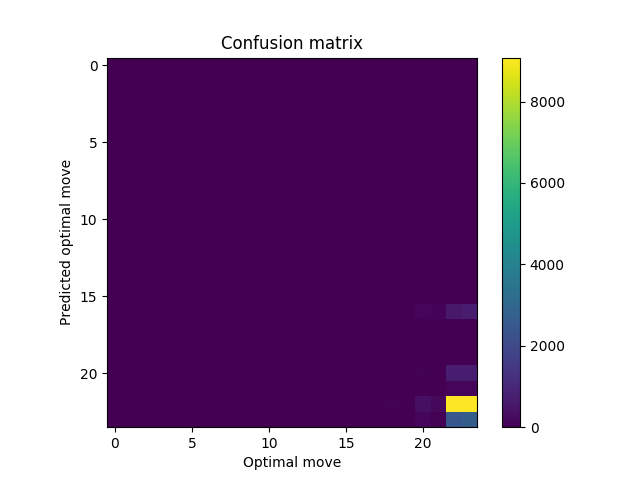
\includegraphics[scale=1]{cm1.png}\\
\caption{DQN Run 1 confusion matrix}
\label{fig:dqn_r1_1}
\end{figure}

\begin{figure}
\centering
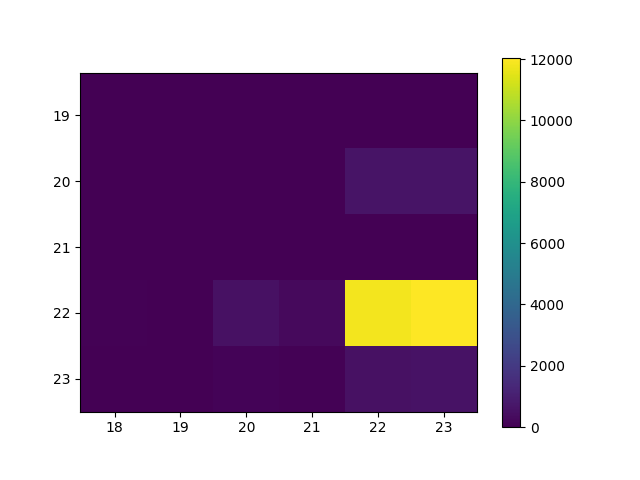
\includegraphics[scale=0.6]{cm3.png}\\
\caption{DQN Run 2 confusion matrix}
\label{fig:dqn_r2_1}
\end{figure}

As most of the variation in the matrix is at the bottom right, we present the close up visualization of that section here \ref{fig:dqn_r1_2} and \ref{fig:dqn_r2_2}

\begin{figure}
\centering
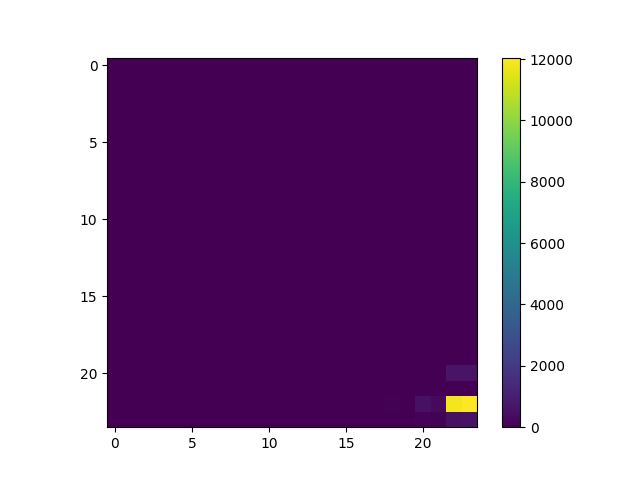
\includegraphics[scale=1]{cm2.png}\\
\caption{DQN Run 1 confusion matrix closeup}
\label{fig:dqn_r1_2}
\end{figure}

\begin{figure}
\centering
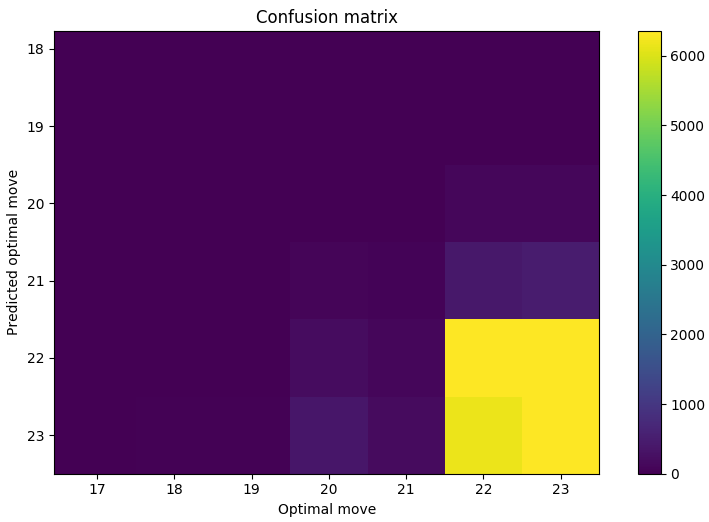
\includegraphics[scale=0.6]{cm4.png}\\
\caption{DQN Run 2 confusion matrix closeup}
\label{fig:dqn_r2_2}
\end{figure}

The acutal values used for heatmap are also presented here, due to most of the upper half not having any special variation, we truncated it and presented here \ref{lst:confusion_matrix}.

\begin{lstlisting}[caption=Confusion matrix for DQN classificaiton, label={lst:confusion_matrix}]
[[   0    0    0    0    0    0    0    0    0    0    0    1    0]
 [   0    0    0    0    0    0    0    0    0    0    0   16   13]
 [   0    0    0    0    0    0    0    0    0    0    0   18    5]
 [   0    0    0    0    0    0    0    0    0    0    0   13   12]
 [   0    0    0    0    0    0    0    0    0    0    0   12   13]
 [   0    0    0    0    0    0    0    0    0    0    0   17    6]
 [   0    0    0    0    0    0    0    0    0    0    0    9    9]
 [   0    0    0    0    0    0    0    0    0    0   10   21   49]
 [   0    0    0    0    0    0    0    0    0    3    4   13   26]
 [   0    0    0    0    0    0    0    1    0   18   77  213  374]
 [   0    0    0    0    0    0    0    0    0   19   69  118  195]
 [   0    0    2    0    0    0    0    0    0  116  406 6347 6167]
 [   0    0    1    0    0    0    0    6    0  113  476 6338 6355]]
\end{lstlisting}
While the data was highly biased towards the last $2$ orderings, our predictions on the otherhand were comparatively diverse.


\subsection{Analysis}
A label based analysis is obtained by using $"\text{metrics.classification\_report}"$ from scikit-learn \cite{scikit-learn}.\\
\begin{lstlisting}[caption=Statistics for various orderings]
             precision    recall  f1-score   support

           9      0.000     0.000     0.000         1
          12      0.000     0.000     0.000        29
          13      0.000     0.000     0.000        23
          14      0.000     0.000     0.000        25
          15      0.000     0.000     0.000        25
          16      0.000     0.000     0.000        23
          17      0.000     0.000     0.000        18
          18      0.000     0.000     0.000        80
          19      0.000     0.000     0.000        46
          20      0.067     0.026     0.038       683
          21      0.066     0.172     0.096       401
          22      0.483     0.487     0.485     13038
          23      0.481     0.478     0.479     13289

   micro avg      0.462     0.462     0.462     27681
   macro avg      0.084     0.089     0.084     27681
weighted avg      0.461     0.462     0.461     27681
\end{lstlisting}
\textbf{Precision}, for each class is the ratio of the number of data entries correctly predicted in this category to the number of data points predicted to be of this class. So the above can be the precision column can be interpreted as:-
\begin{itemize}
    \item For ordering $23$, of the data points predicted to have the optimal ordering as $23$, $48.1\%$ actually had it as the optimal ordering.
    \item For ordering $22$, of the data points predicted to have the optimal ordering as $22$, $48.3\%$ actually had it as the optimal ordering.
    \item For ordering $21$, of the data points predicted to have the optimal ordering as $21$, $6.6\%$ actually had it as the optimal ordering.
\end{itemize} 

\textbf{Recall}, for each class if the ratio of the number of data points correctly predicted to have this class to the number of data points which actually had this as the optimal ordering. So in the above table, the recall column can be interpreted as:-
\begin{itemize}
    \item For ordering $23$, of all the data points which had ordering $23$ as their optimal ordering, we predicted $47.8\%$ to have ordering $23$ as the optimal ordering.
    \item For ordering $22$, of all the data points which had ordering $22$ as their optimal ordering, we predicted $48.7\%$ to have ordering $22$ as the optimal ordering.
    \item For ordering $21$, of all the data points which had ordering $21$ as their optimal ordering, we predicted $17.2\%$ to have ordering $21$ as the optimal ordering.
\end{itemize} 

\textbf{F1-score}, for any classification system, it is desirable to have high precision and recall while not overfitting. \textbf{F1-score}  for a class, is the harmonic mean of precision and recall. It aims to give preference to neither precision nor recall. All the various metrics aim to capture various information from the confusion matrix. F1 score is better measure when False negatives and False positives are important and if there is a class imbalance.
\par \textbf{Micro F1} is calculated by calculating \textbf{micro precision} and \textbf{micro recall} and taking their harmonic mean.\\
\textbf{Micro Precision} is calculated by adding True positive values across all the classes and adding False positives across all classes and treating them as new true positive and false positives to calculate precision.\\
\textbf{Micro Recall} is calculated by adding True positive values across all the classes and adding False negatives across all classes and treating them as new true positive and false negatives to calculate precision.
\par \textbf{Macro F1} is a simple arithmetic mean of f1 scores of all the classes.\\
\textbf{Macro Precision} is a simple arithmetic mean of precisions of all the classes.\\
\textbf{Macro Recall} is a simple arithmetic mean of recalls of all the classes.
\par \textbf{Weighted F1} is weighted arithmetic mean of f1 scores across all classes, with the class strength as weight.\\
\textbf{Weighted Precision} is weighted arithmetic mean of precisions across all classes, with the class strength as weight.\\
\textbf{Weighted Recall} is weighted arithmetic mean of f1 recalls across all classes, with the class strength as weight.
\subsection{Performance}
From the confusion matrix, we calculate the sum of true positives across all the classes. We see that $12978$ data points had predictions correct out of $27681$ data points, that is around $47\%$. While the total accuracy isn't very high, looking solely at the number of correct predictions isn't enough, as we are more interested in the improvement in performance offered by this model.
\par Below we have few examples of our predictions. The bar chart shows the number of operations required by each ordering, the predicted optimal ordering is in red. \ref{fig:operations1} and \ref{fig:operations2}

\begin{figure}
\centering
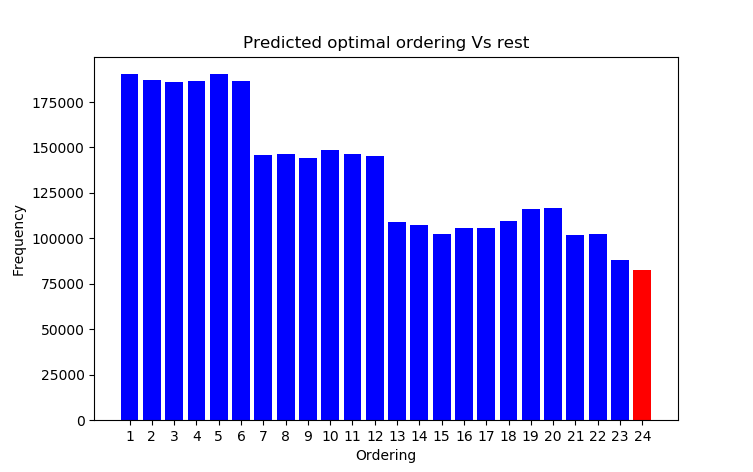
\includegraphics[scale=0.8]{operations1.png}\\
\caption{The figure shows the log$_{10}$(number of operations) required to execute the query depending on the ordering of the selection operators chosen. The predicted optimal ordering is shown in red.}
\label{fig:operations1}
\end{figure}

\begin{figure}
\centering
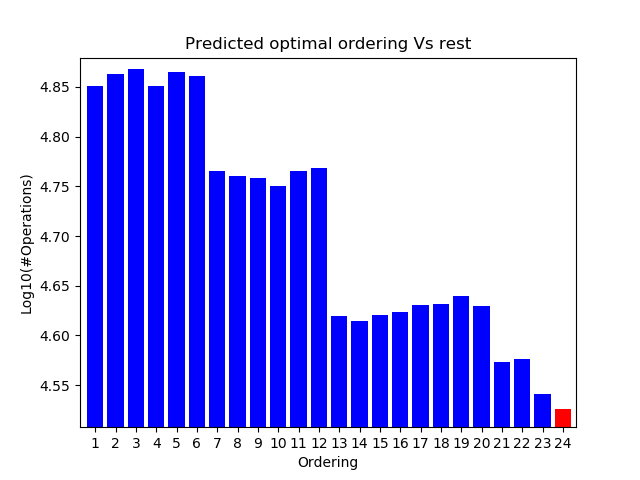
\includegraphics[scale=0.8]{operations2.png}\\
\caption{The figure shows the log$_{10}$(number of operations) required to execute the query depending on the ordering of the selection operators chosen. The predicted optimal ordering is shown in red.}
\label{fig:operations2}
\end{figure}

\par Given that we have the numbr of operations required to be executed by each ordering, we can look at the sum of number of operations of the orders predicted by our model.\\ 
We have the actual optimal ordering, the actual worst ordering, the predicted best ordering from the model.\\
We add the number of operations required by following each of the above $3$ and look at the sum of them.
\begin{itemize}
    \item The sum of operations required by the optimal ordering $890640075.0$
    \item The sum of operations required by the predicted ordering $900269878.0$
    \item The sum of operations required by the optimal ordering $2310227856.0$
\end{itemize}
This tells us that our predicted orderings required approximately $39\%$ operations of the number of operations required by the worst ordering executed always and $102\%$ operations of the number operations required by the best ordering executed always.\\

\section{Discussion}
Learning from data streams is a continuous process. The learning systems that act in dynamic environments, where working conditions change and evolve, need to monitor their working conditions. They need to monitor the learning process  for change detection, emergence of novel classes, changes in the relevance of features, changes in the optimal parameters  settings, and others \cite{DNN_for_stream}.\\
We divide this section into the following parts:-
\begin{itemize}
    \item \textbf{Interpretations} We will interpret the above stated results and see what they mean.
    \item \textbf{Implications} Why do these results matter and what can they lead to.
    \item \textbf{Limitations} the limitations we experienced in the experiments carried out in this thesis.
\end{itemize}


\subsection{Interpretations}
Despite the biased input data classes, the final strategy we got from the DQN gave us a performance of $101\%$ of the optimal solution, we can safely say, DQN have proved to be useful in this case. The successive epoches of DQN also can be seen to improve the results via the diagram.\\
But contrary to the expected result, the number of data points for which we were able to predict to optimal move correctly are roughly $48\%$, the lack of accuracy across the $24$ classes is concerning which can perhaps be addressed to the lack of features used in training the DQN.\\
Overall the improvement of optimal strategy selection is inline with the powerful nature of deep neural networks and iterative nature of reinforcement learning. The high amount of data available from data streams can definitely be a huge plus point for online training methods for DQN for query optimization.\\


\subsection{Implications}
The fact that the application of DQN improved performance by to such a margin, serves to prove that DQNs can be applied in at least some cases for optimizing queries on data stream. Methods for using DQN for query optimization on static data are shown here \cite{drl_dbms} and we use it as an motivation to apply it on data streams.  \\
This makes a strong case for further work in this field, application of deep reinforcement learning to optimize query processing on stream data, to explore more SQL like implementation and integration of the DQN model along with online learning feature.\\
As we saw in this experiment, we achieved a model which tells us an strategy for ordering which requires only $1\%$ more operations than the optimal ordering. Application of DQN on other queries can similarly provide a huge speed up and perhaps reduction in resources consumed. \\
It is popular in recent AI research to try end-to-end learning, where problems that were traditionally factored into subproblems (e.g., self-driving cars involve separate modelsfor localization, obstacle detection and lane-following) are learned in a single unified model. One can imagine a similar architectural ambition for an end-to-end learning query optimizer, which simply maps subplan features to measured runtimes. Thiis would require a significant corpus of run-time data to learn from, and changes to the featurization and perhaps the deep network structure we used here. DQ is a pragmatic middle ground that exploits the structure of the join optimization problem\cite{drl_dbms}.

\subsection{Limitations}
The work presented in this thesis has a number of limitations.
\begin{itemize}
    \item The neural network is unable to achieve low loss for the test data, this perhaps speak the lack of features extracted during the querying time.
    \item The data sample we have is highly biased, leading to rather baised DQNs.
    \item The entire method need to be parallelized and set up on a scalable infrastructure to see the actual effects of DQN.
    \item The DQN used is simulating a single move game rather than a multi move game.
    \item Not looked at how DQNs can be trained online.
\end{itemize}


\section{Conclusion}
In this chapter we saw :-
\begin{itemize}
    \item The method for selecting the optimal move and the assumption for it.
    \item The classificaiton of the data and how it is split between training and testing.
    \item Analyzed and visualized the confusion matrix on different runs of DQN.
    \item The performance of the DQN on predicting.
\end{itemize}
In the next chapter we:-
\begin{itemize}
    \item Present the overall results of the thesis.
    \item Present the take aways.
    \item Present the ways of improving upon this work.
\end{itemize}
%1.2 change to research problem. Most important, 1.4
%Typing error, grammar
